% SPDX-License-Identifier: AGPL-3.0-or-later
% Copyright (C) 2019-2024 Andrew Rechnitzer
% Copyright (C) 2022-2024 Colin B. Macdonald

\documentclass[12pt]{exam}

%%%%%%%%%%%%%%%%%%%%%%%%%%%%%%%%%%%%%%%%%%%%%%%%%%%%
%% This template uses latex exam class.
%%
%% This template is for letter-paper, not a4 paper.
%% The margins have been set so as to work nicely
%% with the QR-codes etc needed by Plom.
%%
%% It has also been designed to use the latex exam class
%% which auto-computes totals etc and also makes it easy
%% for the instructor to include solutions in their .tex
%% We recommend that you use this.

%%%%%%%%%%%%%%%%%%%%%%%%%%%%%%%
%% To print answers/soln and remove the extra spacing
%% just comment out the line below
%% vvvvv
%% vvv
%% v

% \printanswers%

%% ^
%% ^^^
%% ^^^^^
%% Try running this with and without the line above
%%%%%%%%%%%%%%%%%%%%%%%%%%%%%%%%%%%%%%%%%%%%%%%%%%%%
%% Add "draft" to show mock-up QR codes
%\usepackage{mockplom}
%\usepackage[draft]{mockplom}
%%%%%%%%%%%%%%%%%%%%%%%%%%%%%%%%%

\boxedpoints        % puts boxes around the score for each question
\marksnotpoints     % call scores 'marks' not 'points'
\addpoints          % total up the marks for each question 
\extrawidth{-20mm}  % control margins for plom-qr-code positioning.

%%%%%%%%%%%%%%%%%%%%%%%%%%%%%%%%%%%%%%%%%%%%%%%%%%%%

% A simple warning for your Do-Not-Mark pages
\newcommand{\dnm}{\noindent%
\emph{Please do not write on this page --- it will not be marked.}%
}

% Here are some handy commands for adding spacing / blank pages / answerboxes
% when printing with or without solns.

% Use the command below to put a vfill between things when printing
% without answers/solutions. No space when printing with answers/solns
\newcommand{\blank}{ \ifprintanswers{}\else{\vfill}\fi }

% Use the command below to put a blankpage when printing without answers/solutions.
% No page when printing with answers/solns
% This takes an optional argument of a question-number: \blankpage[X]
% and prints a message telling the student that this blank space is for
% question X. If no arg given then it prints the same message but for
% the current question. Thanks to PDL for improving this.
\newcommand{\blankpage}[1][\thequestion]{%
\ifprintanswers{}\else{\par\vfill\newpage%
\noindent \emph{This blank page is for your solution to \textbf{Question~{#1}} if you need more space.}%
\par\vfill\newpage}\fi%
}

% Use this to make a nice answerbox which will display the correct answer
% when solutions are printed and is otherwise blank for the students
% to write their stuff.
\newcommand{\answerbox}[1]{%
\begin{flushright}\fbox{\parbox[l]{60mm}{Answer: \ifprintanswers{#1}\else{\vspace{10mm}}\fi}}\end{flushright}%
}
% A slightly larger answerbox
\newcommand{\Answerbox}[1]{%
\begin{flushright}\fbox{\parbox[l]{80mm}{Answer: \ifprintanswers{#1}\else{\vspace{10mm}}\fi}}\end{flushright}%
}

%%%%%%%%%%%%%%%%%%%%%%%%%%%%%%%%%
%% Load packages and things here
\usepackage{amsmath,amsthm,amsfonts,amssymb}
\usepackage{enumerate}
\usepackage{graphicx}
\usepackage{tikz}

%%%%%%%%%%%%%%%%%%%%%%%%%%%%%%%%%
% Use tikz to put a big "Solutions" watermark on the first page 
% if compiled with solutions
% the command takes an optional argument to print a version-number
\newcommand{\watermarkPageIfSolutions}[1][\empty]{
\ifprintanswers%
\begin{tikzpicture}[remember picture, overlay]%
\node [text=red, rotate=55, scale=10, opacity=.25] at (current page.center){%
\ifx\empty{\textsf{SOLUTIONS}}\else{\begin{tabular}{c} \textsf{SOLUTIONS}\\ \textsf{VERSION~#1} \end{tabular}}\fi
};%
\end{tikzpicture}%
\fi%
}

%%%%%%%%%%%%%%%%%%%%%%%%%%%%%%%%%
% Make the header blank, but put page info in the footer.
\chead{}
\cfoot{Page \thepage\ of \numpages}

%%%%%%%%%%%%%%%%%%%%%%%%%%%%%%%%%
%% Your macros should go here
%% for example
\newcommand{\dee}[1]{{\mathrm{d}#1}}
\newcommand{\diff}[2]{\dfrac{\dee{#1}}{\dee{#2}}}

%%%%%%%%%%%%%%%%%%%%%%%%%%%%%%%%%
%% Time to start the actual test

\begin{document}
\watermarkPageIfSolutions[1]
% puts a big red "SOLUTIONS" watermark on the coverpage 
% when you compile with solutions. The optional argument "1"
% means that it will also write "VERSION 1" in the watermark

\section*{Mathematics 418 --- Midterm --- 45 minutes}
\subsection*{3rd September 1752} % an auspicious date
\begin{itemize}
  \item The test consists of \numpages\ pages and \numquestions\ questions worth a total of \numpoints\ marks.
  \item This is a closed-book examination. \textbf{None of the following are allowed}: documents, cheat sheets or electronic devices of any kind (including calculators, phones, smart watches, etc.)
  \item No work on this page will be marked.
  \item Fill in the information below before turning to the questions.
\end{itemize}

\begin{center}
  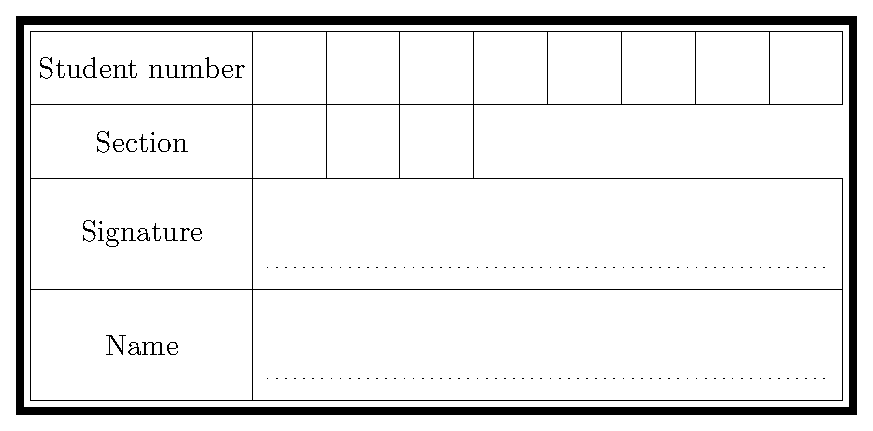
\includegraphics{idBox4}
\end{center}

\vfill

\newpage
% this page consists of instructions and formulas,
% so we use the dnm command to print a message to students
% telling them that nothing on this page will be marked.
\dnm

\subsection*{Additional instructions}
\begin{itemize}
  \item Please use the spaces indicated.
  \item If you require extra paper then put up your hand and ask your instructor.
  \begin{itemize}
    \item You must put your name and student number on any extra pages.
    \item You must indicate the test-number and question-number.
    \item Please do this \textbf{on both sides} of any extra pages.
  \end{itemize}
  \item Please do not dismember your test. You must submit all pages.
  \item Smoking is strictly prohibited during the test.
\end{itemize}

\vfill
\subsection*{Formula sheet}
You may find the following formulas useful in the questions that follow.
\begin{align*}
  a^2 + b^2 &= c^2 \\
  e^{i\pi}+1 &= 0 \\
  \sum_{i=1}^n i &= \frac{n(n+1)}{2} \\
  \diff{}{x}(f+g) &= \diff{f}{x}+\diff{g}{x} \\
  \int (f+g)\dee{x} &= \int f \dee{x} + \int g \dee{x} \\
  \cos(a+b) &= \cos a \cos b - \sin a \sin b \\
  \sin(a+b) &= \sin a \cos b + \cos a \sin b \\
  A \cup (B \cap C) &= (A\cup B) \cap (A \cup C) \\
  A \cap (B \cup C) &= (A\cap B) \cup (A \cap C) \\
  \overline{A \cap B} &= \overline{A} \cup \overline{B} \\
  \overline{A \cup B} &= \overline{A} \cap \overline{B}
\end{align*}
\vfill

\newpage


\begin{questions}
\question[5] Please place your answers in the boxes provided.
\begin{parts}
  \part Find the derivative of $\sin(x^2 y^3)$ with respect to $x$.
  \answerbox{$2xy^3 \cos(x^2 y^3)$}
  \begin{solution}
    We calculate the partial derivative.
    We also need the chain rule.
  \end{solution}
  \blank
  % Use \blank to space out the question parts nicely.

  \part Another little thing here.
  \answerbox{\(\sin(x)\)}
  \begin{solution}
    Putting in your solutions ahead of time really helps calibrate your test.
  \end{solution}
  \blank  % more spacing

  \part A third thing
  \answerbox{\(\int \sin(x) dx\)}
  \begin{solution}
    Yet another solution goes here.
    \[ \int \sin(x) dx = -\cos(x) + C\]
  Note--- (-1) if no \(+C\)
  \end{solution}
  \blank % and yet more spacing.
\end{parts}
\newpage

%% Next question

\question[5]
Please place your answers in the boxes provided.
\begin{parts}
  \part Answer something not quite so simple
  \answerbox{ABC}
  \begin{solution}
    Some working will go here. Like the question, the solution will not be so simple and may span several lines, and have some rubric information for the marker to use.
  \end{solution}
  \blank
  % Use \blank to space out the question parts nicely.

  \part Another less simple thing here.
  \answerbox{\(\sin(x)\)}
  \begin{solution}
    Putting in your solutions ahead of time really helps calibrate your test. If the answer is \(\sin(x)\) what was the question?
  \end{solution}
  \blank

  \part A third thing unsimple thing here.
  \answerbox{\(\int \sin(x) dx\)}
  \begin{solution}
    Yet another solution goes here. This one looks similar to a previous solution. Maybe there is a subtle difference in the solution which we should really make very clear to the grader (and student) here.
  \end{solution}
  \blank
\end{parts}
\newpage

%% Next question

\question[10] A long question goes here. In fact it is sufficiently long that we make sure you have a whole extra blank page for your work.
\begin{solution}
  A long solution here. Maybe it even contains a diagram? A careful diagram is a beautiful thing.
\end{solution}

% The command below creates a blank page and will print a message 
% telling students that the space is for the current question.
\blankpage

\end{questions}
\end{document}
